\begin{landscape}
\chapter{Листинги}
\section{Конфигурационный файл параметров сети Modbus}\label{app:sec:modbus_tag}
    \lstinputlisting[
        language=MyXML,
        caption=Конфигурационный файл для описания множества контроллируемых параетров по промышленному протоколу Modbus
            из раздела \ref{sec:modbus_tag}. Файл разметки приведен в листинге \ref{lst:modbus_tags_example_configs},
        label=lst:modbus_tags_example]
            {Dissertation/listings/xml/modbus_tags_example.xml}
\end{landscape}

\section{Конфигурация сценария}\label{app:sec:modbus_scenario_example_diagram}
\lstinputlisting[
    language=MyXML,
    caption=Конфигурационный файл примера сценария развития событий (см. рисунок \ref{fig:modbus_scenario_example_diagram}),
    label=lst:modbus_scenario_example_diagram]
        {Dissertation/listings/xml/modbus_tags_example_scenario.xml}

\begin{landscape}
\section{\todo{XSD} файлы}\label{app:sec:xsd}
    \lstinputlisting[
        language=MyXML,
        caption=\todo{modbus scheme},
        label=lst:modbus_tags_example_configs]
            {Dissertation/listings/xsd/modbus_tags_configs.xsd}
    
    \lstinputlisting[
        language=MyXML,
        caption=\todo{modbus scenario scheme},
        label=lst:modbus_tags_scenario_configs]
            {Dissertation/listings/xsd/modbus_tags_scenario_configs.xsd}        
\end{landscape}

\chapter{Свидетельство о государственной регистрации программы для ЭВМ}\label{ch:app1}
\todo{Свидетельство и акт я получу на работе.}
\begin{center}
    \begin{figure}[hb]
        
\includegraphics[width=.7\textwidth]{registration}
        \caption{Скан свидетельства о регистрации}\label{app:fig:registration}
    \end{figure}
\end{center}



\chapter{Акт о внедрении}\label{ch:app2}
\begin{center}
    \begin{figure}[hb]
        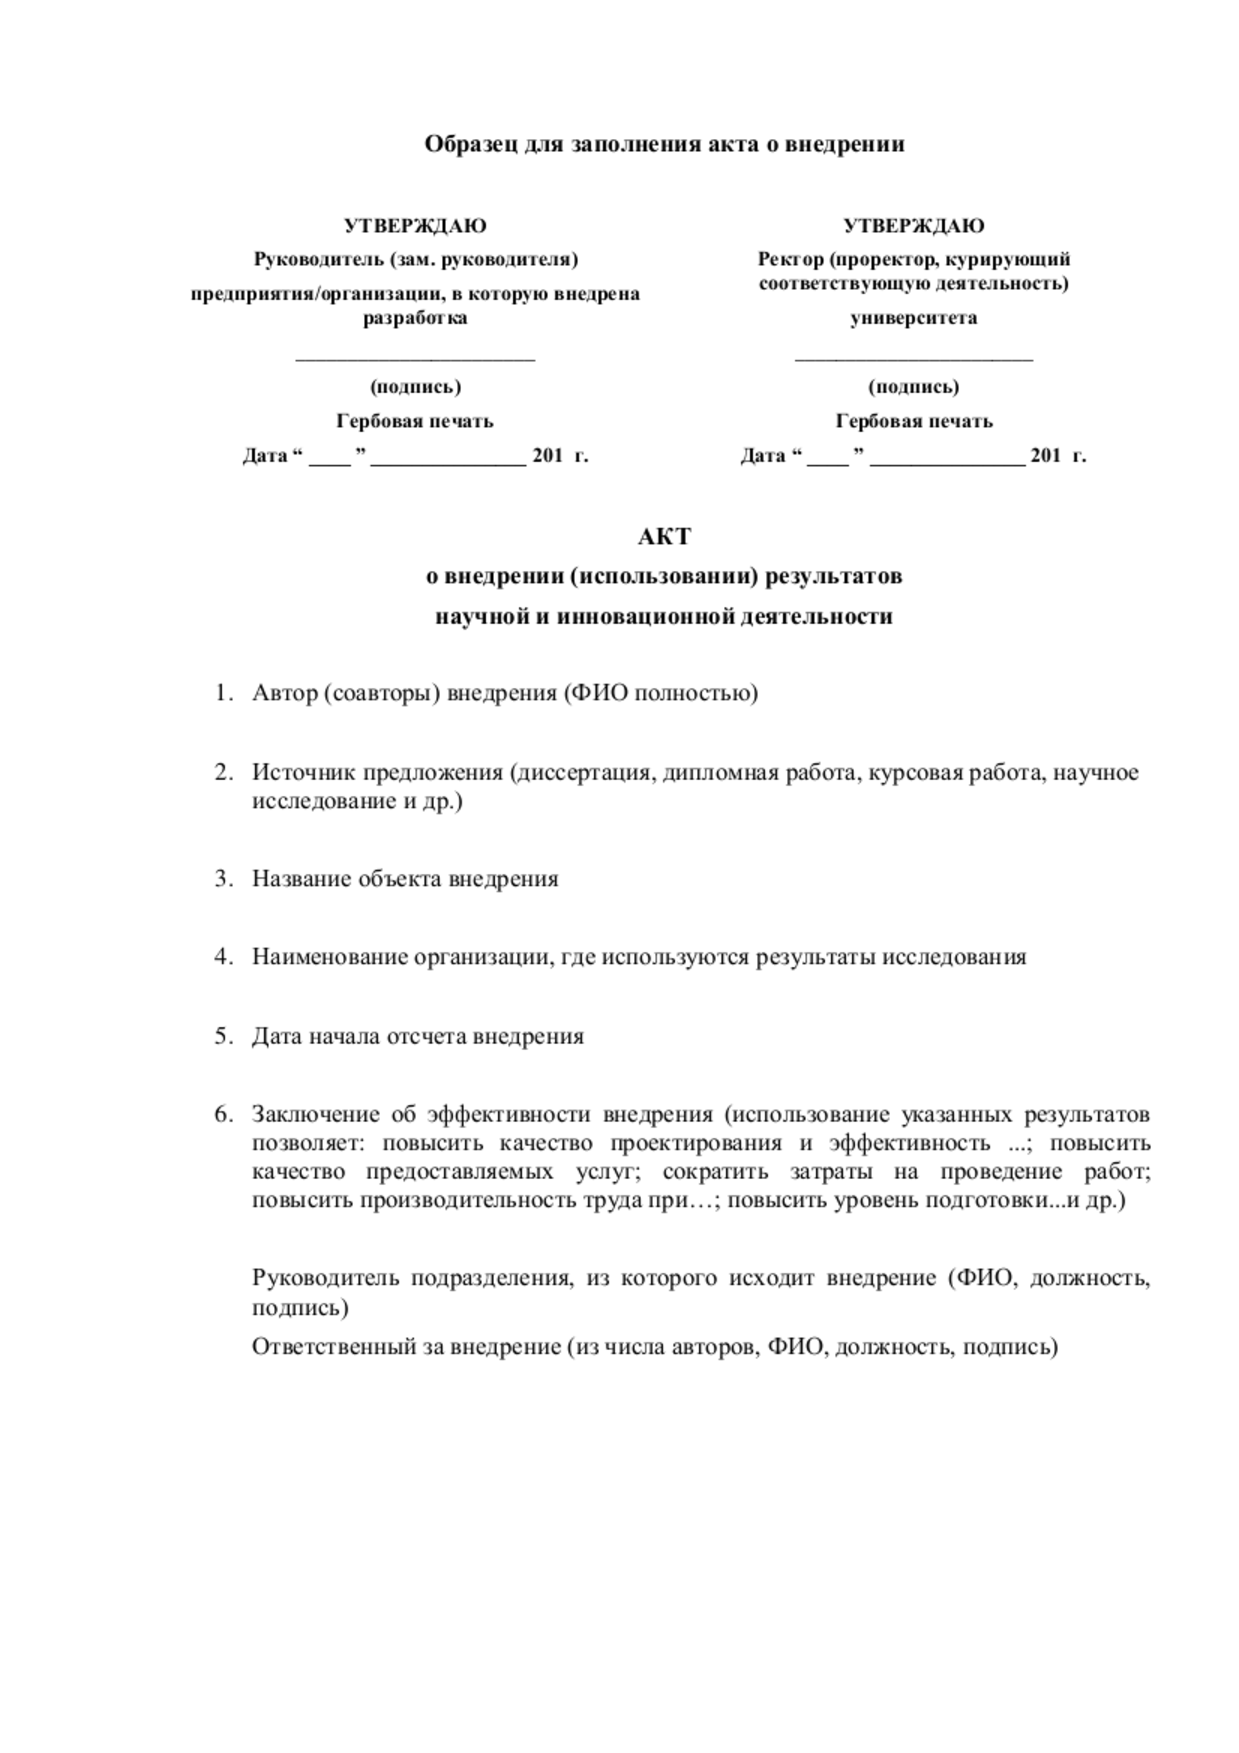
\includegraphics[width=.7\textwidth]{implementation.pdf}
        \caption{Акт о внедрении}\label{app:fig:implementation}
    \end{figure}
\end{center}